\begin{enumerate}[label=\thechapter.\arabic*,ref=\thechapter.\theenumi]
\item Let $\{-1, -\frac{1}{2}, 1, \frac{5}{2}, 3\}$ be a realization of a random sample of size $5$ from a population having $N\left(\frac{1}{2}, \sigma^2\right)$ distribution, where $\sigma > 0$ is an unknown parameter. Let $T$ be an unbiased estimator of $\sigma^2$ whose variance attains the Cramer-Rao lower bound. Then, based on the above data, the realized value of $T$ (rounded off to two decimal places) equals
\hfill (GATE ST 63 2023)
\iffalse
\let\negmedspace\undefined
\let\negthickspace\undefined
\documentclass[journal,12pt,onecolumn]{IEEEtran}
\usepackage{cite}
\usepackage{amsmath,amssymb,amsfonts,amsthm}
\usepackage{algorithmic}
\usepackage{graphicx}
\usepackage{textcomp}
\usepackage{xcolor}
\usepackage{txfonts}
\usepackage{listings}
\usepackage{enumitem}
\usepackage{mathtools}
\usepackage{gensymb}
\usepackage[breaklinks=true]{hyperref}
\usepackage{tkz-euclide} % loads  TikZ and tkz-base
\usepackage{listings}



\newtheorem{theorem}{Theorem}[section]
\newtheorem{problem}{Problem}
\newtheorem{proposition}{Proposition}[section]
\newtheorem{lemma}{Lemma}[section]
\newtheorem{corollary}[theorem]{Corollary}
\newtheorem{example}{Example}[section]
\newtheorem{definition}[problem]{Definition}
%\newtheorem{thm}{Theorem}[section] 
%\newtheorem{defn}[thm]{Definition}
%\newtheorem{algorithm}{Algorithm}[section]
%\newtheorem{cor}{Corollary}
\newcommand{\BEQA}{\begin{eqnarray}}
\newcommand{\EEQA}{\end{eqnarray}}
\newcommand{\define}{\stackrel{\triangle}{=}}
\theoremstyle{remark}
\newtheorem{rem}{Remark}
%\bibliographystyle{ieeetr}
\begin{document}
%
\providecommand{\pr}[1]{\ensuremath{\Pr\left(#1\right)}}
\providecommand{\prt}[2]{\ensuremath{p_{#1}^{\left(#2\right)} }}        % own macro for this question
\providecommand{\qfunc}[1]{\ensuremath{Q\left(#1\right)}}
\providecommand{\sbrak}[1]{\ensuremath{{}\left[#1\right]}}
\providecommand{\lsbrak}[1]{\ensuremath{{}\left[#1\right.}}
\providecommand{\rsbrak}[1]{\ensuremath{{}\left.#1\right]}}
\providecommand{\brak}[1]{\ensuremath{\left(#1\right)}}
\providecommand{\lbrak}[1]{\ensuremath{\left(#1\right.}}
\providecommand{\rbrak}[1]{\ensuremath{\left.#1\right)}}
\providecommand{\cbrak}[1]{\ensuremath{\left\{#1\right\}}}
\providecommand{\lcbrak}[1]{\ensuremath{\left\{#1\right.}}
\providecommand{\rcbrak}[1]{\ensuremath{\left.#1\right\}}}
\newcommand{\sgn}{\mathop{\mathrm{sgn}}}
\providecommand{\abs}[1]{\left\vert#1\right\vert}
\providecommand{\res}[1]{\Res\displaylimits_{#1}} 
\providecommand{\norm}[1]{\left\lVert#1\right\rVert}
%\providecommand{\norm}[1]{\lVert#1\rVert}
\providecommand{\mtx}[1]{\mathbf{#1}}
\providecommand{\mean}[1]{E\left[ #1 \right]}
\providecommand{\cond}[2]{#1\middle|#2}
\providecommand{\fourier}{\overset{\mathcal{F}}{ \rightleftharpoons}}
\newenvironment{amatrix}[1]{%
  \left(\begin{array}{@{}*{#1}{c}|c@{}}
}{%
  \end{array}\right)
}
%\providecommand{\hilbert}{\overset{\mathcal{H}}{ \rightleftharpoons}}
%\providecommand{\system}{\overset{\mathcal{H}}{ \longleftrightarrow}}
	%\newcommand{\solution}[2]{\textbf{Solution:}{#1}}
\newcommand{\solution}{\noindent \textbf{Solution: }}
\newcommand{\cosec}{\,\text{cosec}\,}
\providecommand{\dec}[2]{\ensuremath{\overset{#1}{\underset{#2}{\gtrless}}}}
\newcommand{\myvec}[1]{\ensuremath{\begin{pmatrix}#1\end{pmatrix}}}
\newcommand{\mydet}[1]{\ensuremath{\begin{vmatrix}#1\end{vmatrix}}}
\newcommand{\myaugvec}[2]{\ensuremath{\begin{amatrix}{#1}#2\end{amatrix}}}
\providecommand{\rank}{\text{rank}}
\providecommand{\pr}[1]{\ensuremath{\Pr\left(#1\right)}}
\providecommand{\qfunc}[1]{\ensuremath{Q\left(#1\right)}}
	\newcommand*{\permcomb}[4][0mu]{{{}^{#3}\mkern#1#2_{#4}}}
\newcommand*{\perm}[1][-3mu]{\permcomb[#1]{P}}
\newcommand*{\comb}[1][-1mu]{\permcomb[#1]{C}}
\providecommand{\qfunc}[1]{\ensuremath{Q\left(#1\right)}}
\providecommand{\gauss}[2]{\mathcal{N}\ensuremath{\left(#1,#2\right)}}
\providecommand{\diff}[2]{\ensuremath{\frac{d{#1}}{d{#2}}}}
\providecommand{\myceil}[1]{\left \lceil #1 \right \rceil }
\newcommand\figref{Fig.~\ref}
\newcommand\tabref{Table~\ref}
\newcommand{\sinc}{\,\text{sinc}\,}
\newcommand{\rect}{\,\text{rect}\,}
%%
%	%\newcommand{\solution}[2]{\textbf{Solution:}{#1}}
%\newcommand{\solution}{\noindent \textbf{Solution: }}
%\newcommand{\cosec}{\,\text{cosec}\,}
%\numberwithin{equation}{section}
%\numberwithin{equation}{subsection}
%\numberwithin{problem}{section}
%\numberwithin{definition}{section}
%\makeatletter
%\@addtoreset{figure}{problem}
%\makeatother

%\let\StandardTheFigure\thefigure
\let\vec\mathbf

\bibliographystyle{IEEEtran}


\vspace{3cm}



\bigskip

\renewcommand{\thefigure}{\theenumi}
\renewcommand{\thetable}{\theenumi}
%\renewcommand{\theequation}{\theenumi}
Q: Let $\{-1, -\frac{1}{2}, 1, \frac{5}{2}, 3\}$ be a realization of a random sample of size $5$ from a population having $N\left(\frac{1}{2}, \sigma^2\right)$ distribution, where $\sigma > 0$ is an unknown parameter. Let $T$ be an unbiased estimator of $\sigma^2$ whose variance attains the Cramer-Rao lower bound. Then, based on the above data, the realized value of $T$ (rounded off to two decimal places) equals
\\ \solution
\fi
\begin{definition}
Unbiased Estimator is defined as
\begin{align}
\text{E}(\hat{\sigma^2}) = {\sigma^2}
\end{align}
where, \(E(\hat{\sigma^2})\) represents the expected value of the estimator \(\hat{\sigma^2}\) and \(\sigma^2\) represents the true parameter
\end{definition}
\begin{definition}
The Cramér-Rao bound can be defined as follows:
\begin{align}
\text{Var}(\sigma^2) \geq \frac{1}{I(\sigma^2)}
\end{align}
where $I(\sigma^2)$ represents fisher information for the parameter $\sigma^2$.
Mathematically,
\begin{equation*}
I(\sigma^2) = -E\left [\frac{\partial^2}{\partial(\sigma)^2}\log P_{X}(X|\sigma^2)\right]
\end{equation*}
where, $E[\cdot]$ represents the expected value and $P_{X}(X|\sigma^2)$ is the p.d.f of random variable $X$ given the parameter $\sigma^2$. 
\end{definition}
$P_X(X|\sigma^2)$ is given by:
\begin{align}
P_X(X|\sigma^2) &= \frac{1}{2\pi\sigma^2} \exp\left(-\frac{(X-\frac{1}{2})^2}{2\sigma^2}\right)\\
\log p_X(X|\sigma^2) &= \log\left(\frac{1}{2\pi\sigma^2} \exp\left(-\frac{(X-\frac{1}{2})^2}{2\sigma^2}\right)\right)\\
&= -\frac{1}{2}\log(2\pi\sigma^2) - \frac{(X-\frac{1}{2})^2}{2\sigma^2}\\
\frac{\partial^2}{\partial(\sigma^2)^2}\log P_X(X|\sigma^2) &= \frac{1}{2\pi\sigma^2} - \frac{3(X-\frac{1}{2})^2}{\sigma^4}\\
I(\sigma^2) &= \frac{3}{\sigma^4} E[X^2] - \frac{3}{\sigma^4} E[X] + \frac{3}{4\sigma^4} - \frac{1}{2\pi\sigma^2}\\
E[X^2] &= \sigma^2 + \left(\frac{1}{2}\right)^2\\
E[X] &= \frac{1}{2}\\
\implies I(\sigma^2) &= \left(3 - \frac{1}{2\pi}\right) \frac{1}{\sigma^2}
\end{align}
Hence, Cramér-Rao bound is given as $\frac{\sigma^2}{\left(3 - \frac{1}{2\pi}\right)}$
\begin{definition}
Variance of $T$ attains Cramer-Rao lower bound\\
\(\implies\) $T$ has attained minimum possible variance and $T$ is an efficient estimator
\end{definition}
\begin{table}[h!]
 \begin{center}
    \begin{tabular}{|c|c|c|c|c|c|}
    \hline
    $X_i$ & -1 & $-\frac{1}{2}$ & 1 & $\frac{5}{2}$ & 3\\
    \hline
    $({X_i} - \mu)^{2}$ & $\frac{9}{4}$ & 1 & $\frac{1}{4}$ & 4 & $\frac{25}{4}$\\
    \hline
    \end{tabular}
    \end{center}
    \caption{Table 1}
  \label{tab:GATE/2023/ST/63/} 
\end{table}
Therefore,
\begin{align}
T &= \frac{\sum (X_i - \mu)^{2}}{n}\\
n &= 5\\
\mu &= \frac{1}{2}
\end{align}
\begin{align}
\sum (X_i - \mu)^{2} &= 13.75
\end{align}
Hence,
\begin{align}
T &= 2.75
\end{align}
Since, $T$ is an unbiased estimator of $\sigma^2$,
\begin{align}
\text {Cramér-Rao bound} &= \frac{T}{\left(3 - \frac{1}{2\pi}\right)}\\
&= 0.968
\end{align}

\item Let $X$ be a random variable with probability density function
\begin{align}
\label{eq:22/2023/1}f(x;\lambda)&=
\begin{cases}
\frac{1}{\lambda}e^{-\frac{x}{\lambda}} & \text{if} x>0\\
0 & \text{otherwise}
\end{cases}
\end{align}
where $\lambda > 0$ is an unknown parameter. Let $Y_1, Y_2,...,Y_n$ be a random sample of
size $n$ from a population having the same distribution as $X^2$.If
\begin{align}
\label{eq:22/2023/2}\bar{Y} &= \frac{1}{n}\sum_{i=1}^n Y_i
\end{align}
then which of the following statements is true?
\begin{enumerate}
\item \label{eq:22/2023/3}$\sqrt{\frac{\bar{Y}}{2}} \text{is a method of moments estimator of}         \lambda$
\item $\sqrt{\bar{Y}} \text{is a method of moments estimator of}\lambda$
\item ${\frac{1}{2}\sqrt{\bar{Y}}} \text{is a method of moments estimator of }\lambda$
\item $2\sqrt{\bar{Y}} \text{is a method of moments estimator of} \lambda$
\end{enumerate}
\hfill(GATE ST 22 2023)\\
\iffalse
\let\negmedspace\undefined
\let\negthickspace\undefined
\documentclass[journal,12pt,twocolumn]{IEEEtran}
\usepackage{cite}
\usepackage{amsmath,amssymb,amsfonts,amsthm}
\usepackage{algorithmic}
\usepackage{graphicx}
\usepackage{textcomp}
\usepackage{xcolor}
\usepackage{txfonts}
\usepackage{listings}
\usepackage{enumitem}
\usepackage{mathtools}
\usepackage{gensymb}
\usepackage[breaklinks=true]{hyperref}
\usepackage{tkz-euclide} % loads  TikZ and tkz-base
\usepackage{listings}
\usepackage{gvv}
\documentclass{article}	% working
\def\inputGnumericTable{}
\usepackage[latin1]{inputenc}
\usepackage{fullpage}
\usepackage{color}
\usepackage{array}
\usepackage{longtable}
\usepackage{calc}
\usepackage{multirow}
\usepackage{hhline}
\usepackage{ifthen}
%
%\usepackage{setspace}
%\usepackage{gensymb}
%\doublespacing
%\singlespacing
\usepackage{graphicx}
%\usepackage{amssymb}
%\usepackage{relsize}
%\usepackage[cmex10]{amsmath}
%\usepackage{amsthm}
%\interdisplaylinepenalty=2500
%\savesymbol{iint}
%\usepackage{txfonts}
%\restoresymbol{TXF}{iint}
%\usepackage{wasysym}
%\usepackage{amsthm}
%\usepackage{iithtlc}
%\usepackage{mathrsfs}
%\usepackage{txfonts}
%\usepackage{stfloats}
%\usepackage{bm}
%\usepackage{cite}
%\usepackage{cases}
%\usepackage{subfig}
%\usepackage{xtab}
%\usepackage{longtable}
%\usepackage{multirow}
%\usepackage{algorithm}
%\usepackage{algpseudocode}
%\usepackage{enumitem}
%\usepackage{mathtools}
%\usepackage{tikz}
%\usepackage{circuitikz}
%\usepackage{verbatim}
%\usepackage{tfrupee}
%\usepackage{stmaryrd}
%\usetkzobj{all}
%   \usepackage{color}                                            %%
%    \usepackage{array}                                            %%
%    \usepackage{longtable}                                        %%
%    \usepackage{calc}                                             %%
%    \usepackage{multirow}                                         %%
%    \usepackage{hhline}                                           %%
%    \usepackage{ifthen}                                           %%
%  optionally (for landscape tables embedded in another document): %%
%    \usepackage{lscape}     
%\usepackage{multicol}
%\usepackage{chngcntr}
%\usepackage{enumerate}
%\usepackage{wasysym}
%\documentclass[conference]{IEEEtran}
%\IEEEoverridecommandlockouts
% The preceding line is only needed to identify funding in the first footnote. If that is unneeded, please comment it out.

\newtheorem{theorem}{Theorem}[section]
\newtheorem{problem}{Problem}
\newtheorem{proposition}{Proposition}[section]
\newtheorem{lemma}{Lemma}[section]
\newtheorem{corollary}[theorem]{Corollary}
\newtheorem{example}{Example}[section]
\newtheorem{definition}[problem]{Definition}
%\newtheorem{thm}{Theorem}[section] 
%\newtheorem{defn}[thm]{Definition}
%\newtheorem{algorithm}{Algorithm}[section]
%\newtheorem{cor}{Corollary}
\newcommand{\BEQA}{\begin{eqnarray}}
\newcommand{\EEQA}{\end{eqnarray}}
\newcommand{\define}{\stackrel{\triangle}{=}}
\theoremstyle{remark}
\newtheorem{rem}{Remark}

%\bibliographystyle{ieeetr}
\begin{document}
%

\bibliographystyle{IEEEtran}


\vspace{3cm}

\title{
%	\logo{
Assignment

\Large{EE23010: Probability and Random Processes}\\
Indian Institute of Technology,Hyderabad
%	}
}
\author{ Aman Kumar 

EE22BTECH11006
}	
		%\title{
%	\logo{Matrix Analysis through Octave}{\begin{center}\includegraphics[scale=.24]{tlc}\end{center}}{}{HAMDSP}
%}


% paper title
% can use linebreaks \\ within to get better formatting as desired
%\title{Matrix Analysis through Octave}
%
%
% author names and IEEE memberships
% note positions of commas and nonbreaking spaces ( ~ ) LaTeX will not break
% a structure at a ~ so this keeps an author's name from being broken across
% two lines.
% use \thanks{} to gain access to the first footnote area
% a separate \thanks must be used for each paragraph as LaTeX2e's \thanks
% was not built to handle multiple paragraphs
%

%\author{<-this % stops a space
%\thanks{}}
%}
% note the % following the last \IEEEmembership and also \thanks - 
% these prevent an unwanted space from occurring between the last author name
% and the end of the author line. i.e., if you had this:
% 
% \author{....lastname \thanks{...} \thanks{...} }
%                     ^------------^------------^----Do not want these spaces!
%
% a space would be appended to the last name and could cause every name on that
% line to be shifted left slightly. This is one of those "LaTeX things". For
% instance, "\textbf{A} \textbf{B}" will typeset as "A B" not "AB". To get
% "AB" then you have to do: "\textbf{A}\textbf{B}"
% \thanks is no different in this regard, so shield the last } of each \thanks
% that ends a line with a % and do not let a space in before the next \thanks.
% Spaces after \IEEEmembership other than the last one are OK (and needed) as
% you are supposed to have spaces between the names. For what it is worth,
% this is a minor point as most people would not even notice if the said evil
% space somehow managed to creep in.



% The paper headers
%\markboth{Journal of \LaTeX\ Class Files,~Vol.~6, No.~1, January~2007}%
%{Shell \MakeLowercase{\textit{et al.}}: Bare Demo of IEEEtran.cls for Journals}
% The only time the second header will appear is for the odd numbered pages
% after the title page when using the twoside option.
% 
% *** Note that you probably will NOT want to include the author's ***
% *** name in the headers of peer review papers.                   ***
% You can use \ifCLASSOPTIONpeerreview for conditional compilation here if
% you desire.




% If you want to put a publisher's ID mark on the page you can do it like
% this:
%\IEEEpubid{0000--0000/00\$00.00~\copyright~2007 IEEE}
% Remember, if you use this you must call \IEEEpubidadjcol in the second
% column for its text to clear the IEEEpubid mark.



% make the title area
\maketitle

\newpage

%\tableofcontents

\bigskip

\renewcommand{\thefigure}{\theenumi}
\renewcommand{\thetable}{\theenumi}
%\renewcommand{\theequation}{\theenumi}

%\begin{abstract}
%%\boldmath
%In this letter, an algorithm for evaluating the exact analytical bit error rate  (BER)  for the piecewise linear (PL) combiner for  multiple relays is presented. Previous results were available only for upto three relays. The algorithm is unique in the sense that  the actual mathematical expressions, that are prohibitively large, need not be explicitly obtained. The diversity gain due to multiple relays is shown through plots of the analytical BER, well supported by simulations. 
%
%\end{abstract}
% IEEEtran.cls defaults to using nonbold math in the Abstract.
% This preserves the distinction between vectors and scalars. However,
% if the journal you are submitting to favors bold math in the abstract,
% then you can se LaTeX's standard command \boldmath at the very start
% of the abstract to achieve this. Many IEEE journals frown on math
% in the abstract anyway.

% Note that keywords are not normally used for peerreview papers.
%\begin{IEEEkeywords}
%Cooperative diversity, decode and forward, piecewise linear
%\end{IEEEkeywords}



% For peer review papers, you can put extra information on the cover
% page as needed:
% \ifCLASSOPTIONpeerreview
% \begin{center} \bfseries EDICS Category: 3-BBND \end{center}
% \fi
%
% For peerreview papers, this IEEEtran command inserts a page break and
% creates the second title. It will be ignored for other modes.
%\IEEEpeerreviewmaketitle

Question: Let $X$ be a random variable with probability density function
\begin{align}
\label{eq:22/2023/1}f(x;\lambda)&=
\begin{cases}
\frac{1}{\lambda}e^{-\frac{x}{\lambda}} & \text{if} x>0\\
0 & \text{otherwise}
\end{cases}
\end{align}
where $\lambda > 0$ is an unknown parameter. Let $Y_1, Y_2,...,Y_n$ be a random sample of
size $n$ from a population having the same distribution as $X^2$.If
\begin{align}
\label{eq:22/2023/2}\bar{Y} &= \frac{1}{n}\sum_{i=1}^n Y_i
\end{align}
then which of the following statements is true?
\begin{enumerate}
\item \label{eq:22/2023/3}$\sqrt{\frac{\bar{Y}}{2}} \text{is a method of moments estimator of}         \lambda$
\item $\sqrt{\bar{Y}} \text{is a method of moments estimator of}\lambda$
\item ${\frac{1}{2}\sqrt{\bar{Y}}} \text{is a method of moments estimator of }\lambda$
\item $2\sqrt{\bar{Y}} \text{is a method of moments estimator of} \lambda$
\end{enumerate}
\hfill(GATE ST 2023)\\
\fi
\solution
\begin{enumerate}
\item Using PDF in \eqref{eq:22/2023/1} we need to find an estimator for the unknown parameter $\lambda$ in terms of sample mean $\bar{Y}$\\
we know $Y_i=X_i^2$
then,
\begin{align}
E(Y_i)&=E(X_i^2)\\
&= \int_{0}^{\infty}x^2\frac{1}{\lambda}e^{-\frac{x}{\lambda}}\\
&= 2{\lambda}^2
\end{align} 
Method of moment is defined by \eqref{eq:22/2023/2} which gives,
\begin{align}
\bar{Y} & = E(Y_i)\\
&= 2{\lambda}^2
\end{align} 
where
\begin{align}
\lambda &= \sqrt{\frac{\bar{Y}}{2}}
\end{align}
$\therefore$ Option \eqref{eq:22/2023/3} is correct.
\item The simulation steps to estimate $\lambda$ using method of moment estimator in python.
\begin{enumerate}
\item Generate a random value of $\lambda$ within the specified range using \textbf{np.random.uniform(1,10)}
\item Use the generated $\lambda$ to create a random sample of $X$ values following the given PDF using \textbf{np.random.exponential()}
\item Then, generate $Y$ as $Y=X^2$ 
\item calculate the mean ($\bar{Y}$) as \textbf{np.mean($Y$)}
\item Hence, the estimated value of $\lambda$ is \textbf{np.sqrt($\frac{\bar{Y}}{2}$)}
\end{enumerate}
\end{enumerate}
Graph of simulated CDF vs Theoretical CDF
\begin{figure}[ht]
	\centering
	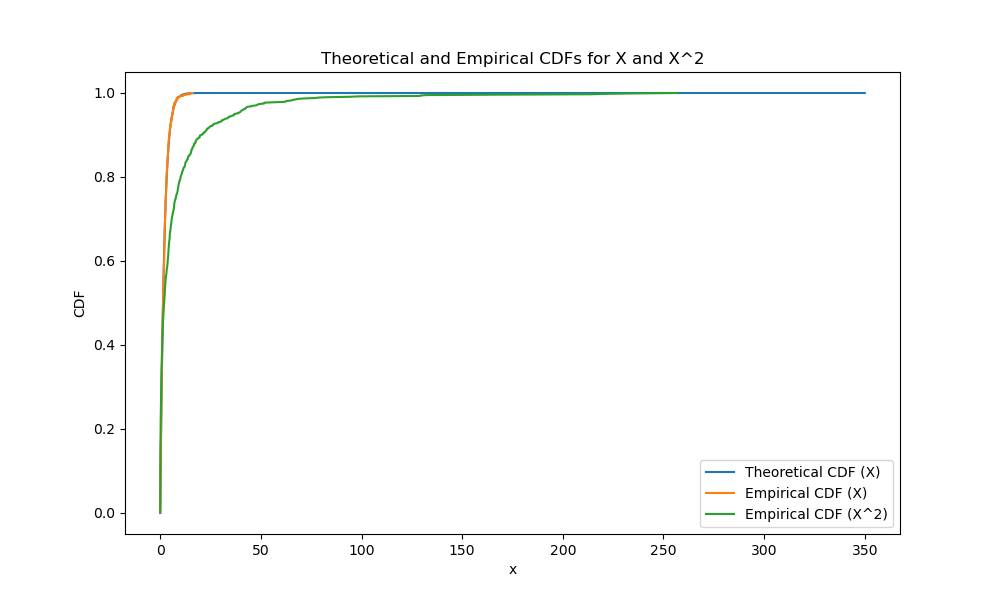
\includegraphics[width=\columnwidth]{2023/ST/22/figs/fig.png}
    \caption{Figure1}
	\label{Fig:Figure1}
\end{figure}

\end{enumerate}
